\subsection{Room sizes}
\label{sec:application:building_the_model:room_sizes}

In the seventh step, a field referencing the new enumeration type is introduced. \cref{subsec:library_of_transformations:type_level_transformations:enum_fields} is used to introduce the enumeration field on the type level, while on the instance level, \cref{subsec:library_of_transformations:instance_level_transformations:enum_field_values} is used to introduce the values.

The $classtype$ of the new field is $.\type{Room}$, as the field will be defined for rooms. The $name$ of the new field is $\type{room\_size}$ and the $enumid$ is $.\type{RoomSize}$. Furthermore, the set of $enumvalues$ is equal to the set of values for the $.\type{RoomSize}$ enumeration type, so $enumvalues = \{\type{SMALL}, \type{MEDIUM}, \type{LARGE}\}$. Then, $enumids$ returns for each enumeration value the corresponding node identifier used in the GROOVE graph, while $enumob$ lists the corresponding internal node id.

The set of objects of which the value is set is equal to all room objects, so $objects = \{TRRoom1, TRRoom2, BHPRoomA, BHPRoomB, BHPRoomC\}$. The $values$ function is defined as follows:
\begin{align*}
    values = \{&(TRRoom1, \type{LARGE}), (TRRoom2, \type{MEDIUM}), (BHPRoomA, \type{SMALL}), \\&(BHPRoomB, \type{SMALL}), (BHPRoomC, \type{SMALL})\}
\end{align*}

The following model is obtained:

\LTXtable{\textwidth}{tex/06_application/02_building_the_model/tables/07_room_sizes.tex}

\begin{figure}[p]
    \centering
    \begin{subfigure}{0.98\textwidth}
        \centering
        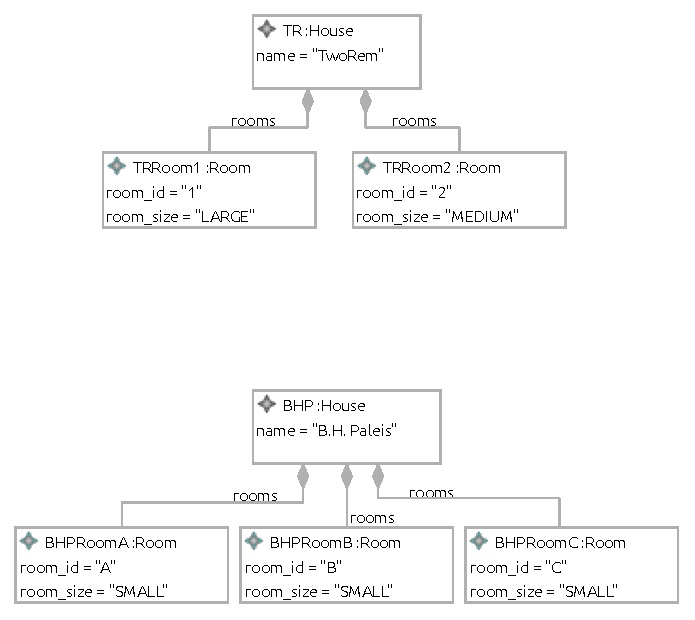
\includegraphics{images/06_application/instance_model/step07.pdf}
        \caption{Instance Model $Im_7$}
        \label{fig:application:building_the_model:room_sizes:ecore:instance_model}
    \end{subfigure}
    \\
    \begin{subfigure}{0.98\textwidth}
        \centering
        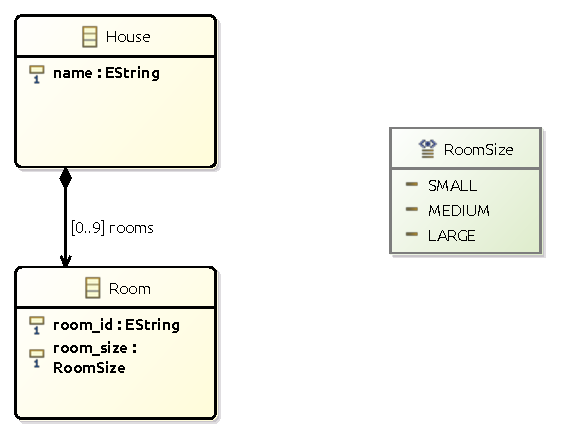
\includegraphics{images/06_application/type_model/step07.pdf}
        \caption{Type Model $Tm_7$}
        \label{fig:application:building_the_model:room_sizes:ecore:type_model}
    \end{subfigure}
    \caption{The Ecore model after step 7}
    \label{fig:application:building_the_model:room_sizes:ecore}
\end{figure}

\begin{figure}[p]
    \centering
    \begin{subfigure}{0.98\textwidth}
        \centering
        % To use this figure in your LaTeX document
% import the package groove/resources/groove2tikz.sty
%
\begin{tikzpicture}[scale=\tikzscale,name prefix=step07-]
\node[type_node] (n0) at (0.740, -0.400) {\ml{\textbf{House}\\name: \textbf{string}}};
\node[type_node] (n1) at (0.730, -1.585) {\ml{\textbf{Room}\\room\_id: \textbf{string}}};
\node[type_node] (n2) at (2.380, -0.560) {\ml{\textbf{RoomSize}\\\textit{LARGE}\\\textit{MEDIUM}\\\textit{SMALL}}};

\path[basic_edge, composite](n0.south -| 0.730, -1.585) -- node[lab] {\ml{rooms}} (n1) ;
\path[basic_edge] (n1)  -- node[lab] {\ml{room\_size}} (n2) ;
\end{tikzpicture}

        \caption{Instance Graph $IG_7$}
        \label{fig:application:building_the_model:room_sizes:groove:instance_graph}
    \end{subfigure}
    \\
    \begin{subfigure}{0.98\textwidth}
        \centering
        % To use this figure in your LaTeX document
% import the package groove/resources/groove2tikz.sty
%
\begin{tikzpicture}[scale=\tikzscale,name prefix=step07-]
\node[type_node] (n0) at (0.740, -0.400) {\ml{\textbf{House}\\name: \textbf{string}}};
\node[type_node] (n1) at (0.730, -1.585) {\ml{\textbf{Room}\\room\_id: \textbf{string}}};
\node[type_node] (n2) at (2.380, -0.560) {\ml{\textbf{RoomSize}\\\textit{LARGE}\\\textit{MEDIUM}\\\textit{SMALL}}};

\path[basic_edge, composite](n0.south -| 0.730, -1.585) -- node[lab] {\ml{rooms}} (n1) ;
\path[basic_edge] (n1)  -- node[lab] {\ml{room\_size}} (n2) ;
\end{tikzpicture}

        \caption{Type Graph $TG_7$}
        \label{fig:application:building_the_model:room_sizes:groove:type_graph}
    \end{subfigure}
    \caption{The GROOVE graphs after step 7}
    \label{fig:application:building_the_model:room_sizes:groove}
\end{figure}

A visual representation of $Tm_7$ and $Im_7$ can be found in \cref{fig:application:building_the_model:room_sizes:ecore}. Similarly, a visual representation of $TG_7$ and $IG_7$ can be found in \cref{fig:application:building_the_model:room_sizes:groove}. Please note that because of the definitions of $f_7(Im_7)$ and $f'_7(IG_7)$, we have that $f_7(Im_7) = IG_7$ and $f'_7(IG_7) = Im_7$. Furthermore, $f_7(Im_7)$ and $f'_7(IG_7)$ are valid mapping functions themselves, such that they can be combined with another mapping function in the next step.

On the instance model level, no surprising elements are introduced. An enumeration field acts like most other attributes within Ecore. However, the visualisation shows how enumeration values are referenced by their instance nodes in the instance graph. The encoding of the field makes use of the presented encoding to emulate enumeration types within GROOVE.

\afterpage{\FloatBarrier}